\chapter{Introduction}
%addcontentsline{toc}{chapter}{Introduction}
%\thispagestyle{empty}


\vspace{1cm}
\section{Development Environments}

The aim of this manual is to guide the user in the first steps of Python, C++, Fortran and Web (HTML/CSS/JavaScript) programming with Visual Studio. When starting to code in any language there are a number of essential concepts that should be perfectly understood and they are not always clear for beginners. We cover some of those concepts in this introduction. 

Three important concepts we must not confuse are \textbf{Compiler}, \textbf{Interpreter} and \textbf{Integrated Development Environment (IDE)}. On the one hand we have Compilers and Interpreters, they are in charge of transforming the code written in a programming language (Fortran for example) into another programming language (the target language). They generally translate the source code from a high-level language (HLL, languages closer to human language and independent of the particular computer where is written) into a low-level language (e.g. assembly language, object code or machine code, those closer to the hardware) in order to create an executable program. While the compiler takes the whole program and translates it at a time and generating an intermediate object code (less memory efficiency), the interpreter takes all the code line by line and performs the compilation and execution simultaneously. On the contrary, when a compiler is used, the execution comes after the compilation. Compilers are generally faster than interpreters but the detection and removal of errors are more difficult since the interpreter allows resuming the translation when the error is fixed. In addition, it is said that the interpretation or compilation of the code are a property of the implementation and not the language. Hence, some programming languages like C, C++ or Fortran are implemented with a compiler while Python make use of an interpreter in one stage of the implementation. 

On the other hand we find IDEs (like Visual Studio). They are a software application that offers some facilities for software development. Some of the functionalities that the IDE provides are a source code editor (similar to a text editor), build automation tools, version management tools, a debugger, intelligent code completion and a long etcetera. It is possible to write programs without an IDE but it is less comfortable specially when too many source codes are involved in the program. This guide explains how to install and start using \textbf{Microsoft Visual Studio} (which accepts 36 different programming languages) and all the necessary tools associated to the mentioned programming languages. Some of these tools are for example the \textbf{Intel\textregistered \hspace{0.1cm}Fortran Compiler} (Parallel Studio XE 2018) or the compiler for C++ (\textbf{Intel\textregistered \hspace{0.1cm}C++ Compiler} or similar) which allow compiling programs. In addition, a Python interpreter, the Visual Micro extension (Arduino projects) and some web tools will be included in the IDE. Please notice that the first thing to install in your computer is the IDE, Visual Studio. Then all the compilers, interpreters and extensions needed are added to the environment so it can recognise the different languages. 

It has been mentioned before that working with an IDE is not mandatory for programming, it is just an useful tool that can make easier the software development. The process of coding can be developed by means of a code editor or a simple text editor, later with the use of the command prompt we can call the compiler/interpreter of our programming language and build any project. Hence, one question that may appear is: What are the differences and advantages of using an IDE instead of a Code Editor? \label{sec:FAQVS}

Apart from the list mentioned, the \textbf{Integrated Development Environment} provides more tools like project manager, deep code analysis to feed auto-completion, support for many programming languages (in the case of Visual Studio), etc. The IDE is where we write the code and convert it into a product, a compiled program, a web app, etc., using a lot of tools and everything in one single program. 

On the contrary, we find \textbf{Code Editors} which are more than text editors since they have enhanced features. When they are optimized for source code editing, they provide syntax highlighting, navigation tools, search possibilities and they are often easily customized. The bottom line is that they are limited to the edition of plain text, they do not compile and debug the code in their nature, however, they accept plug-ins and extensions to imitate the use of an IDE. Finally, a third option would be programming with \textbf{command-line tools}.

In order to break into the world of software development, we consider that an IDE is the proper tool to use. With Microsoft Visual Studio we can program more efficiently thanks to all the tools that it incorporates by default, with no need of adding plug-ins. A powerful file management tool, some really interesting tools like ``Find All References'', ``Go To definition'' or ``Intrinsic Parameter Info'' are some examples of the available utilities that Visual Studio incorporates. We can compile all the languages, manage source codes and navigate through them, manage all the files involved in the project and debug the code with no need of external programs. 

In the IDE, we have access to all the essential tools related to software development just learning how to use one program and we do not need to check the compatibility between the tools used since they are all implemented in the same environment. While the potential of Visual Studio is more remarkable when developing a big software project, it is a really comfortable tool to use even with little projects. It is sometimes said that a Code Editor is going to be very useful with languages that does not need to be compiled (like JavaScript or a static HTML page for example) since they are lighter. On the contrary, languages like Fortran that are being compiled and executed constantly are going to be easily used with an IDE, which offers quickly (and with no need of external plug-ins) these capabilities. This is specially important when our project needs from the pre-process, compilation and linked of a big amount of codes (with an Editor we should do it manually). 

In addition, IDE's often use the \textbf{Make} tool, this is a build automation tool in charge of building the libraries and executable files of our program starting with the source code. It makes use of files called \textbf{Makefiles} where a set of directives are stored specifying how to generate the target program. This tool decides automatically the order of compilation for all the source codes involved in the project by reading the dependencies between them. Furthermore, if we change the source code of a file and rebuild the whole project, the Make tool will update the project by compiling and rebuilding only one file, with no need of building the whole project again. This can be done by reading the modification date of all the files and as a result the process is much faster, specially when the project has a large number of source codes. 

In conclusion, considering the tools offered by Microsoft: Visual Code and Visual Studio, the first one does not offer the same potential (it is a Code Editor) as Visual Studio. That is why we use Visual Studio in this guide. 


\section{Configuration and Project Files/Folders}

\begin{figure}[h]
    \centering
    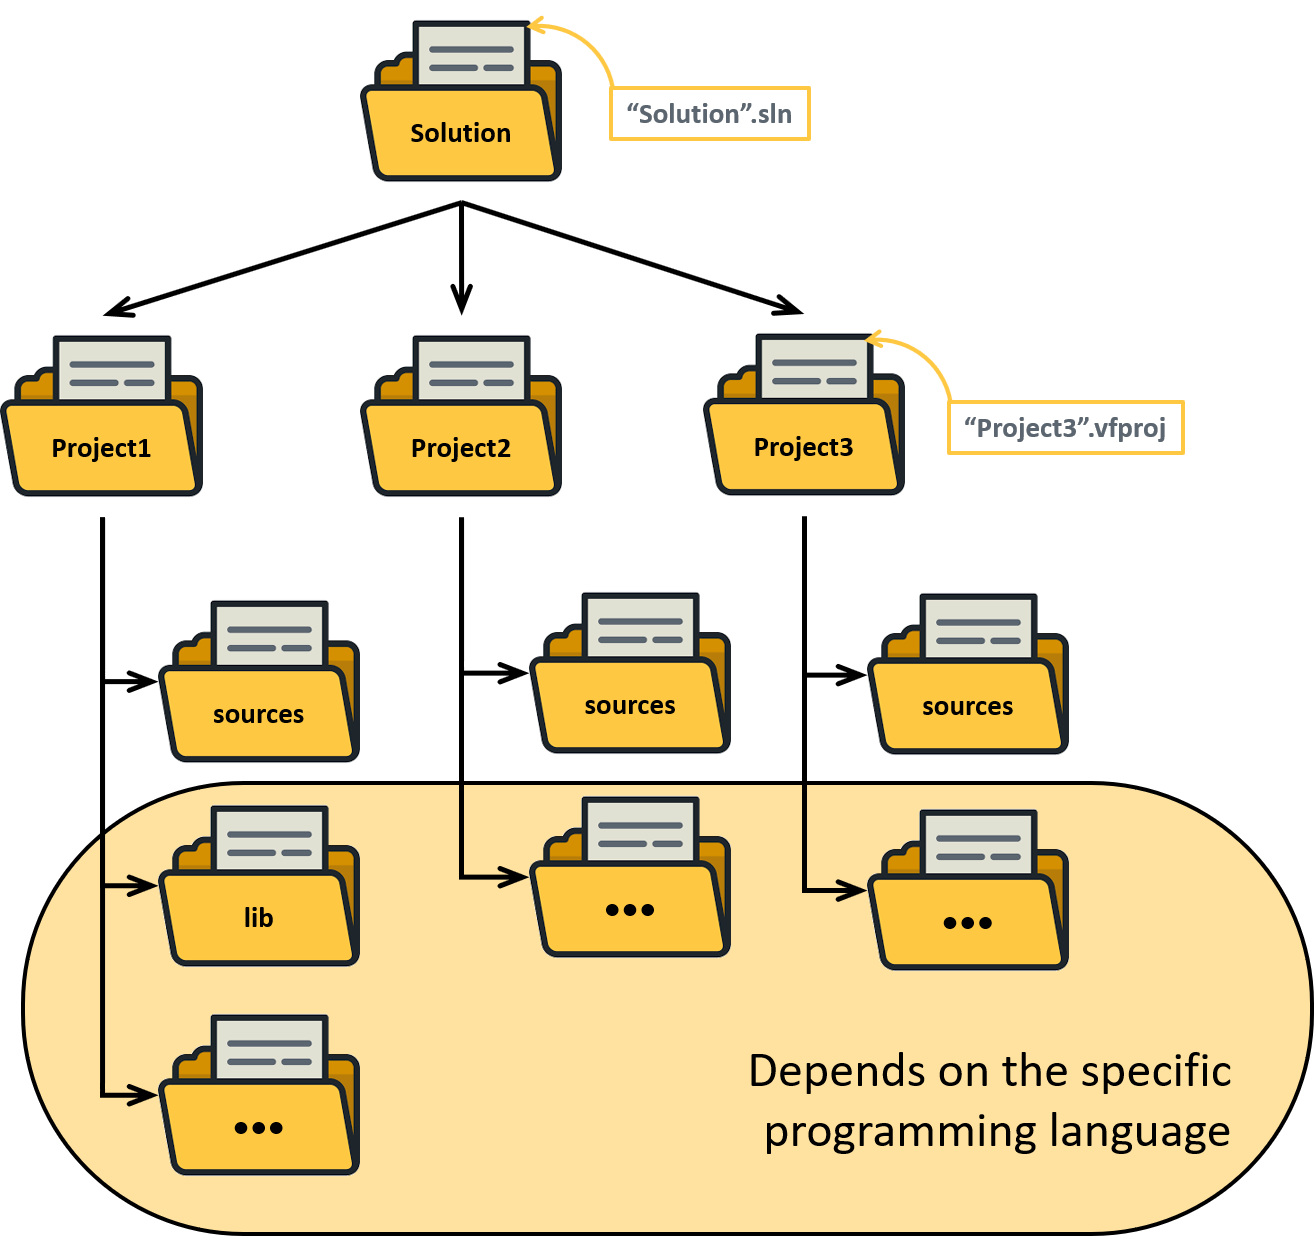
\includegraphics[width= \textwidth]{Figures/FolderScheme}
    \caption{Scheme of the main folders that we should have in a solution containing different projects.}
    \label{fig:FolderScheme}
\end{figure}

A program written in a human-readable programming language with our IDE is not understood by the computer. The Central Processing Unit (CPU) of the computer, in charge of the execution of the program, only processes machine code instructions which reduces the program to a number of very specific tasks in the registers of the CPU itself. The concepts of \textbf{Source} and \textbf{Object Codes} are essential. Both types of codes collect the computer instructions that conform our program. While the source code is written in a human-readable programming language, the object code is generated by the compiler and stores the program in a computer language like machine code (binary for example) or an intermediate language.

The different programming languages that exist store the mentioned codes in different types of files that can be distinguished by the file extension. Just as an example we will see that a source code written in Fortran language is stored in a \texttt{.f90} file while the object code generated by the compiler receives the extension of \texttt{.obj}. In the case of a C++ program, the source code can use the extension \texttt{.cpp} among others and the object code will be stored in the same extension as Fortran language (\texttt{.obj}). Apart from these files, a list of common used extensions can be found in a specific programming language (libraries, modules, images, scripts, etc.), this information is also treated during this guide.

%-----------------------
An important concept to handle is the difference between the \textbf{logical files/folders order} that is generated in our projects and the \textbf{real order} of the files and folders stored in the hard drive. In the first case, we add all the source codes, images, libraries, etc. to the project and we organize all the elements in the Solution explorer of the tool. We can create folders or move files as we want. However, each file can be stored anywhere in our hard drive, maybe in the folder of a different project/solution, in the desktop, in the cloud, etc. This is specially important for languages like Fortran where there is not relation between both schemes. We can add a library file to the logical folder called ``libraries'' while the real file is stored in our Desktop. The Fortran project will store the information about the location of the library. In addition, if we create a new file in that folder (using Visual Studio), it is by default stored in the project folder in the hard drive, but not necessarily in a folder called with the same name. The folders that organize all the necessary content for the program are different and we must manage not only the order used in the solution (seen in the solution explorer in Visual Studio) but also the real location of the files. %This behaviour forces us to know and control at all the time the files/folders structure in our project and the real structure in the hard drive.

It is not the same for languages like Python or JavaScript. Once the project is started, if we create a folder or a code file using Visual Studio, the same folder or file is created in our hard drive in the same location where our project and solution are (both projects and solutions are explained later). In this case we do not have to take an strict control of files since the structure is repeated and consistent. 

Let's think about a code file that we use in many different projects (stored in our desktop, outside our project folder, for example). If we are using Fortran, we can add that file to our project with no need of copying the file to the project folder. Different projects will have the path associated to the file and if we make a modification to the file, all the projects benefit from that update in the next compilation. Once again, this is different for languages like JavaScript. If we add the file to the project, a copy is automatically made in the project folder and a modification in the code stored in the desktop will be totally useless. If the file is used in 3 different projects, a modification in the code can become a mess. We strongly recommend to delete all files that has been previously copied to a project in order to avoid unnecessary duplications (there cannot be two files with the same name). If the code is going to be used in different projects we will build a library with that code (treated in each language) and include it in the different works.

\begin{IN}
    For all these reasons, we are going to follow the same files/folders scheme in our projects from now on. Whether it is automatically created or not, we have to store all the source codes in a folder called ``sources'' inside our folder project (see Figure \ref{fig:FolderScheme}). If the folder is not created by default in both the real and the logical folder scheme, we have to do it manually. In addition, a list of files and folders are created together with the source files in order to make the project work properly. These additional elements depend on the programming language we are using and they would be treated in the specific chapter. As a practical implementation of this topic, take a look at the example \ref{sec:Example2}.
\end{IN}
%-----------------------

Nevertheless, our programs are not only comprised by code files. Visual Studio works with the concepts of projects and solutions, each of them with their \textbf{configuration files and extensions associated}. It is important to clarify the nomenclature that the program gives to the project and solution files since we are going to live together with them from now on. Simplifying, it could be said that a \textit{project} is a specific program written in a programming language while a \textit{solution} is a set of different programs. In the official Microsoft Visual Studio documentation a project is defined as:

\begin{center}
    \begin{minipage}{0.7\linewidth}
        \vspace{3pt}
        {\small
            ``...In a logical sense, a project contains of all the source code files, icons, images, data files and anything else that will be compiled into an executable program or web site, or else is needed in order to perform the compilation. A project also contains all the compiler settings and other configuration files that might be needed by various services or components that your program will communicate with.''
        }
        \begin{flushright}
            (\url{https://msdn.microsoft.com/en-us/library/b142f8e7.aspx})
        \end{flushright}
        \vspace{3pt}
    \end{minipage}
\end{center}

\newpage
Related to solutions, the Visual documentation says: 

\begin{center}
    \begin{minipage}{0.7\linewidth}
        \vspace{3pt}
        {\small
            ``A project is contained, in a logical sense and in the file system, within a solution, which may contain one or more projects, along with build information, Visual Studio window settings, and any miscellaneous files that aren't associated with any project. In a literal sense, the solution is a text file with its own unique format; it is generally not intended to be edited by hand.
            
            A solution has an associated *.suo file that stores settings, preferences and configuration information for each user that has worked on the project.''
        }
        \begin{flushright}
            (\url{https://msdn.microsoft.com/en-us/library/b142f8e7.aspx})
        \end{flushright}
        \vspace{3pt}
    \end{minipage}
\end{center}

%-----------------------

%-----------------------

Both the solution and the project have files associated. The file where the solution is stored has \texttt{.sln} extension and contains information that the environment uses to load it, load the projects within the solution and other information attached. As an example, we can find there the file format version, the newest version of Visual Studio that saved the file, the older version of VS that can open the solution and a list of parameters needed for loading the project files. In the case of the project, the extension of the file depends on the programming language used. If an Intel Fortran project has been created, the extension is \texttt{.vfproj} while in the case of a C++ compiler, \texttt{.icproj} would be the extension. This file stores information about the configuration of the project in the different building modes; Release, Debug and those created by us. It also stores the name and relative path of all the files needed for opening and building the project and the admitted extensions that can be opened. 

The solution and project files are XML files (Extensible Markup Language), this means that the data structure is machine-readable and human-readable at the same time. Although both kind of files are automatically generated by Visual Studio and they are not made for being modified by hand, we can do it if required. We could open the file with a text editor, read the information and change parameters directly with no need of using VS. The solution settings for each user are stored in the \texttt{.suo} file that Visual Studio automatically creates when the solutions is saved. Unlike the mentioned files, this one is stored in a binary format so it is not human-readable and can not be modified by hand. 

All the configuration files mentioned are physically stored in our hard drive, in the folder reserved for the solution and the projects.




\FloatBarrier
\section{Example 1} \label{sec:Ex2}

In order to help the reader in the first steps with Visual Studio, a repository has been created in GitHub with the solutions and projects explained here. Apart from the examples created in the guide, some extra content can be found, specially in the fields of Applied Maths, Simulation software with Fortran, Energy efficiency in buildings or Embedded software (C++). The repository is located in the url: \url{https://github.com/jahrWork} (Figure \ref{fig:repository}).

\begin{figure}
    \centering
    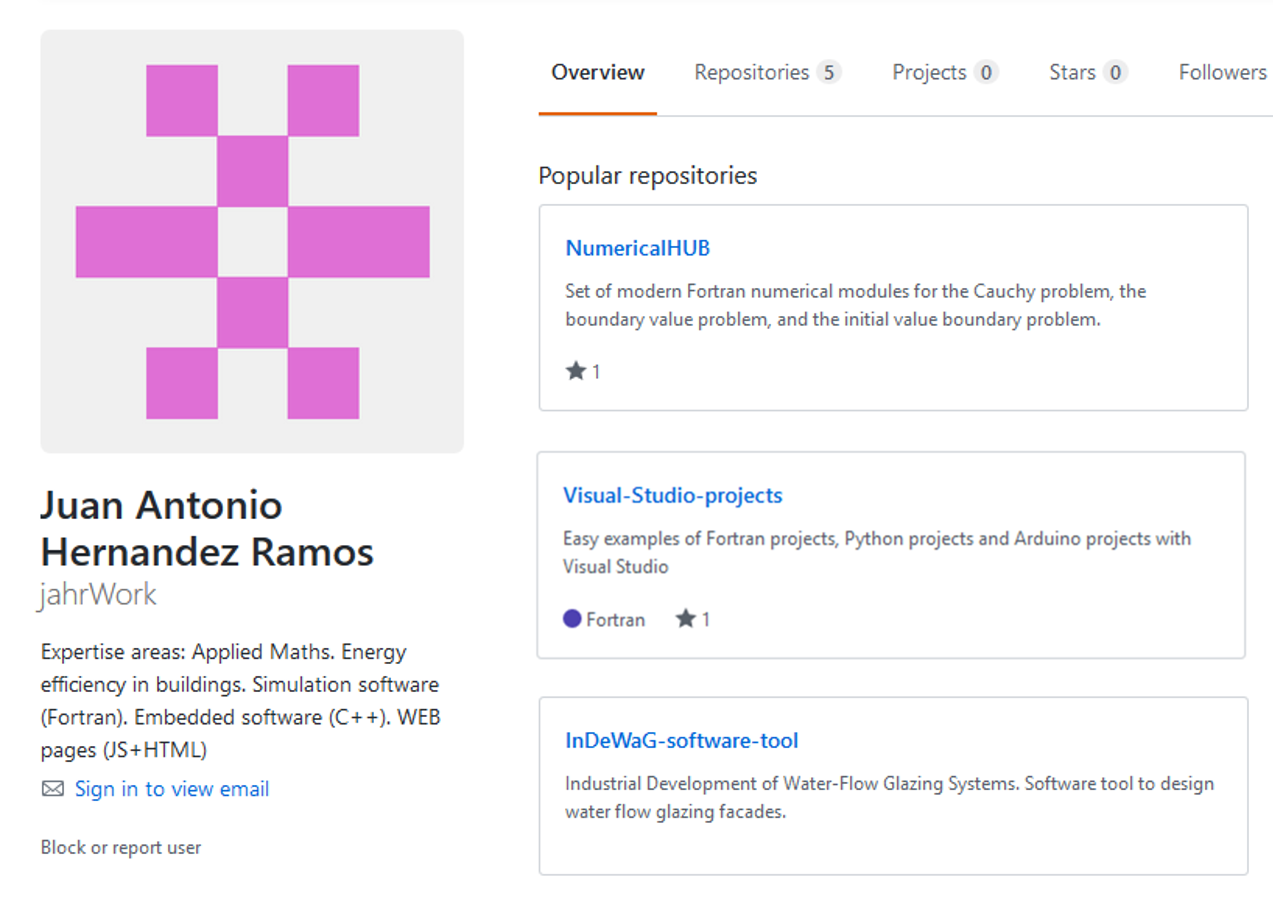
\includegraphics[width= \textwidth]{Figures/repository2}
    \caption{jahrWork repository in GitHub created by Juan Antonio Hernandez Ramos.}
    \label{fig:repository}
\end{figure}

Let's download, open and execute an example of this repository in order to get familiar with the solutions and projects. Follow these steps:

\begin{enumerate}[nosep]
    \item Open the url of the repository in your browser.
    \item Click on \textit{Visual-Studio-projects}.
    \item Click on the green button (\textit{Clone or download}) and click on \textit{Download ZIP}.
    \item In the folder where the ZIP file has been downloaded, unzip the folder and open it. 
    \item Double click on \texttt{Projects.sln} in order to open the solution in Visual Studio. If you just want to open the projects of a specific language, open the folder you want and double click on the \texttt{.sln} file.
    \item You find in the Solution Explorer a mix of projects in different programming languages, make right click on \textit{MainFortranGraph} and click on \textit{Set as StartUp Project} in order to select this project as the execution by default when clicking on the start button.
    \item Click on \textit{BUILD/Build MainFortranGraph} and wait until VS finishes.
    \item Click on \textit{DEBUG/Start Without Debugging} or press \texttt{Ctrl+F5}. The result of the execution is the plot of a sine curve.
\end{enumerate}
 

\FloatBarrier
\section{Example 2} \label{sec:Example2}

It is assumed now that a working version of Visual Studio is already installed in your computer (see chapter \ref{ch:VS}). In this section we create a unique solution called ``Semester1'' and as many projects as milestones have to be completed during the semester. We use Fortran language so the proper compiler must be already installed (see chapter \ref{sec:FortranIns}). The files and folders structure mentioned above is used for this example. 

Follow these steps:

\begin{enumerate}[nosep]
    \item Open your installed version of Visual Studio.
    \item Click on \textit{File/New/Project...} (Figure \ref{fig:Pro1}).
    \item In the \textit{Intel(R) Visual Fortran} menu select \textit{Console Application} and then click on \textit{Main Program Code}.
    \item Write the name of the first project to create in the field \textit{Name}, e.g. ``Milestone1''. Notice that the solution gets the same name by default. 
    \item Change the \textit{Location} of the solution, a directory will be created there.
    \item Write now the name of the solution ``Semester1'', it does not have to be the same as the name of the project (Figure \ref{fig:Intro1}).  
    \item Select the option \textit{Create directory for solution}.
    \item Click on \textit{OK}.
\end{enumerate}

\begin{figure}
    \centering
    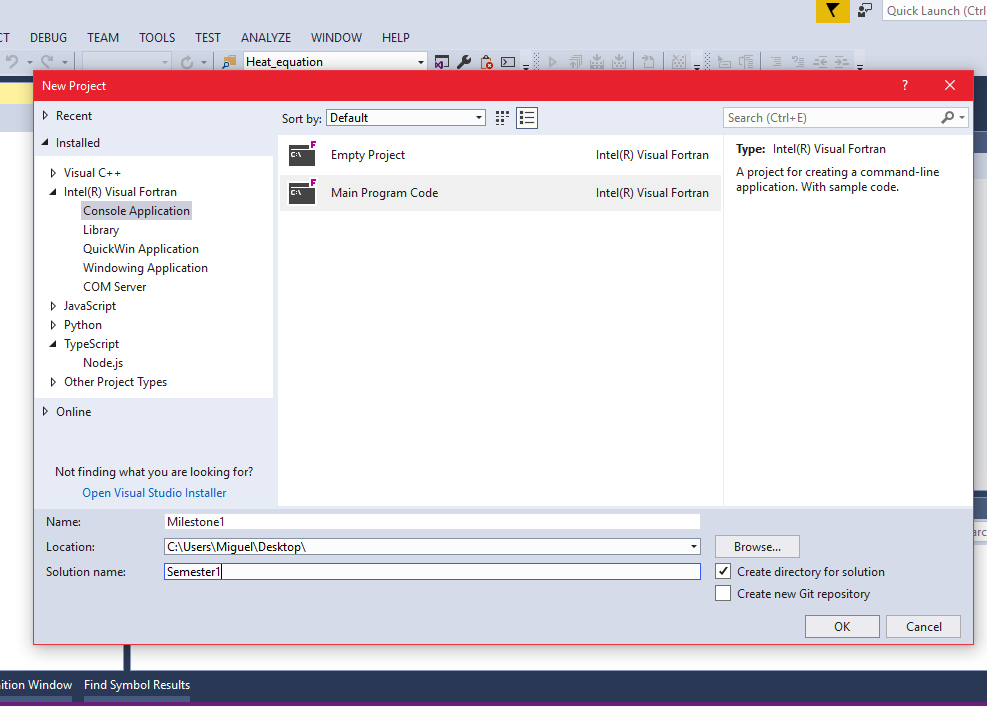
\includegraphics[width= 0.9\textwidth]{Figures/Intro1}
    \caption{Creation of a Fortran project within a solution in Visual Studio.}
    \label{fig:Intro1}
\end{figure}

Open now the path where your new solution has been created and open your solution folder. You find a \texttt{.sln} file with the name ``Semester1'' and a folder \texttt{Milestone1} containing the project data. Right now in this project folder you have a file \texttt{Milestone1.vfproj} with the configuration of the project, this configuration data is read by VS when the solution is opened. In addition, the first source code file \texttt{.f90} (with the same name of the project) has been created.

The folders structure is really different in the Solution Explorer of Visual. Three folders appear inside the project domain: \textit{Header Files}, \textit{Resource Files} and \textit{Source Files}. The last one contains the file \texttt{Milestone1.f90} mentioned above, with the main program code in Fortran (the Figure \ref{fig:Intro2} shows the initial structure of folders and files). In this code the ``Hello World'' example is already written so we can build the project and execute it without debugging. The results will be printed in a command window. 

\begin{figure}
    \centering
    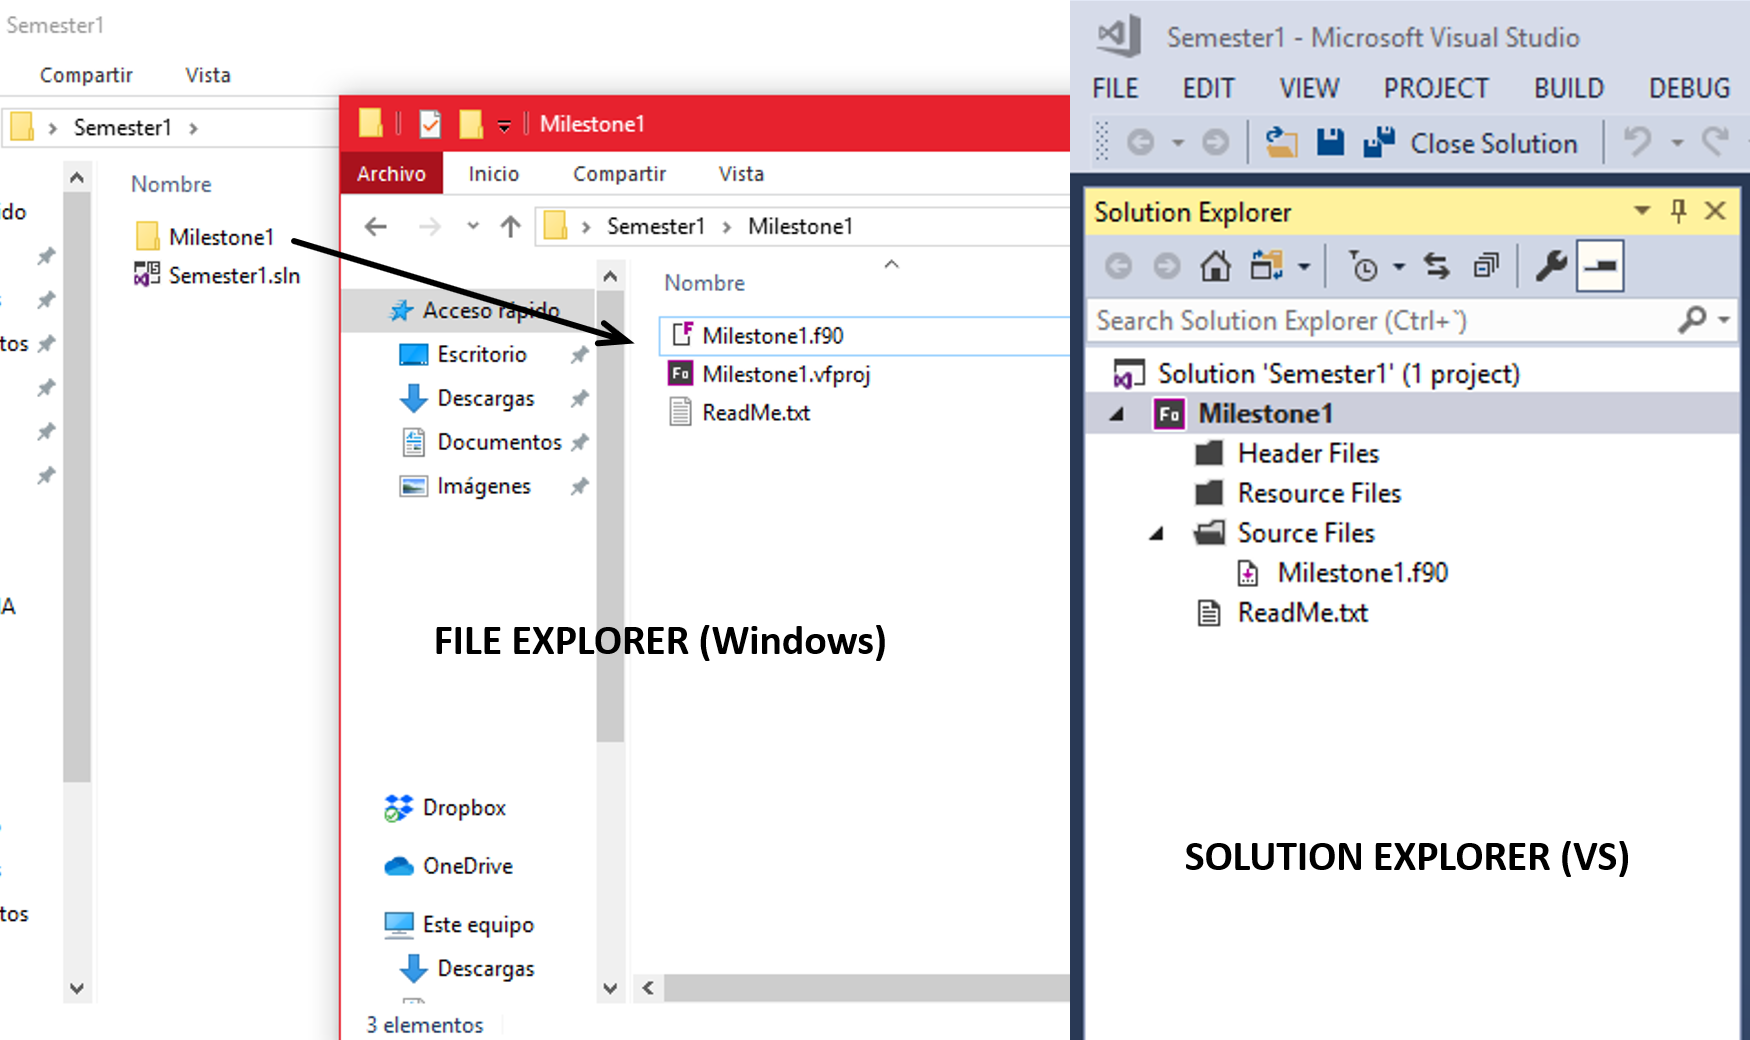
\includegraphics[width= 0.9\textwidth]{Figures/Intro2}
    \caption{Initial folders and files structure in the File Explorer of Windows and the Solution Explorer of Visual Studio.}
    \label{fig:Intro2}
\end{figure}

However, our first project is going to grow and some files and folders will be created. The following steps show how to imitate the structure seen in the Figure \ref{fig:FolderScheme} in order to maintain a strict folder order. 

\begin{enumerate}[nosep]
    \item Open in the File Explorer of Windows OS the project folder:
    
        \texttt{...\textbackslash Semester1\textbackslash Milestone1}.
    
    \item Create there a folder called ``sources''. This folder will contain all the source codes of your program. 
    \item Still using the File Explorer of Windows OS, cut the file \texttt{Milestone1.f90} and paste it inside the recently created folder. The Figure \ref{fig:Intro3} shows the final structure of folders and files.
    \item If you try to open this file in VS (double click on the name of the file in the Solution Explorer of the IDE), you will receive an error since the file is not in the initial location anymore. 
    \item Remove this file in the Solution Explorer by making right click on the name of the file and pressing \textit{Remove} and then clicking on \textit{Remove} once again.
    \item Make right click on the name of the folder \texttt{Source Files} in the Solution Explorer and click on \textit{Add/Existing item...}. Open ``sources'' and select \texttt{Milestone1.f90}. The file is once again in the project but with the new location. 
    \item From now on, all your codes can be stored in the same file ``sources'' (referring to the real order of the files) and they all can be stored in ``Source Files'' (logical order seen by the Solution Explorer). 
\end{enumerate}

Finally, all the projects to be created during the rest of the semester (Milestone2, Milestone3, etc.) can be stored in the same solution. The section \ref{sec:Include} tells how to include new projects and files in a solution already created. At the end of the semester you will have something like the Figure \ref{fig:Intro4}.

\begin{figure}
    \centering
    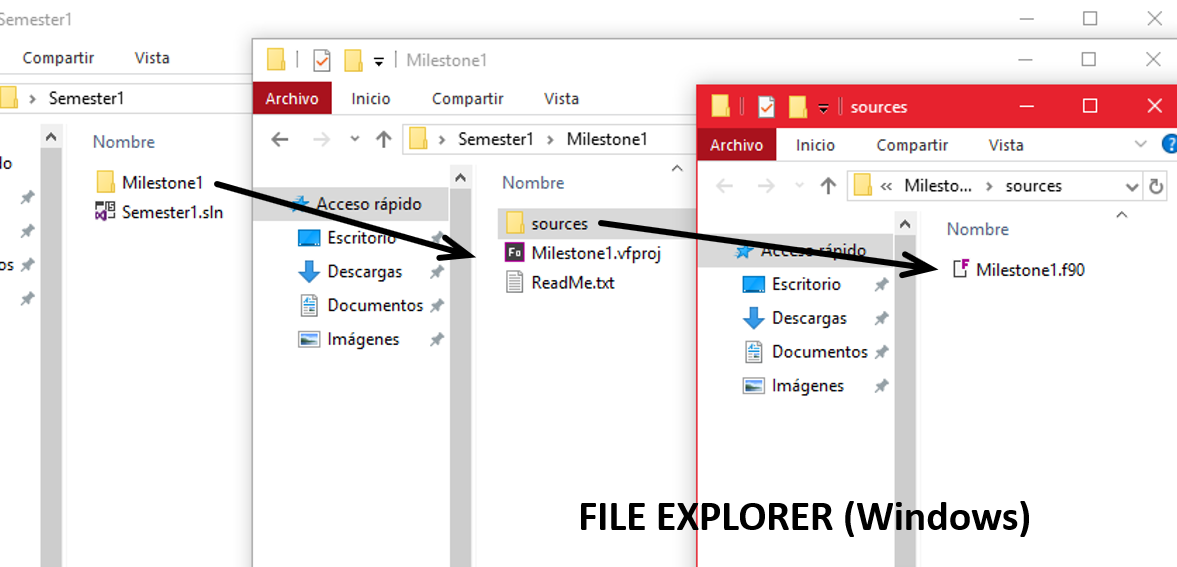
\includegraphics[width=  \textwidth]{Figures/Intro3}
    \caption{Folders and files structure in the File Explorer of Windows after organizing the Fortran project.}
    \label{fig:Intro3}
\end{figure}

\begin{figure}
    \centering
    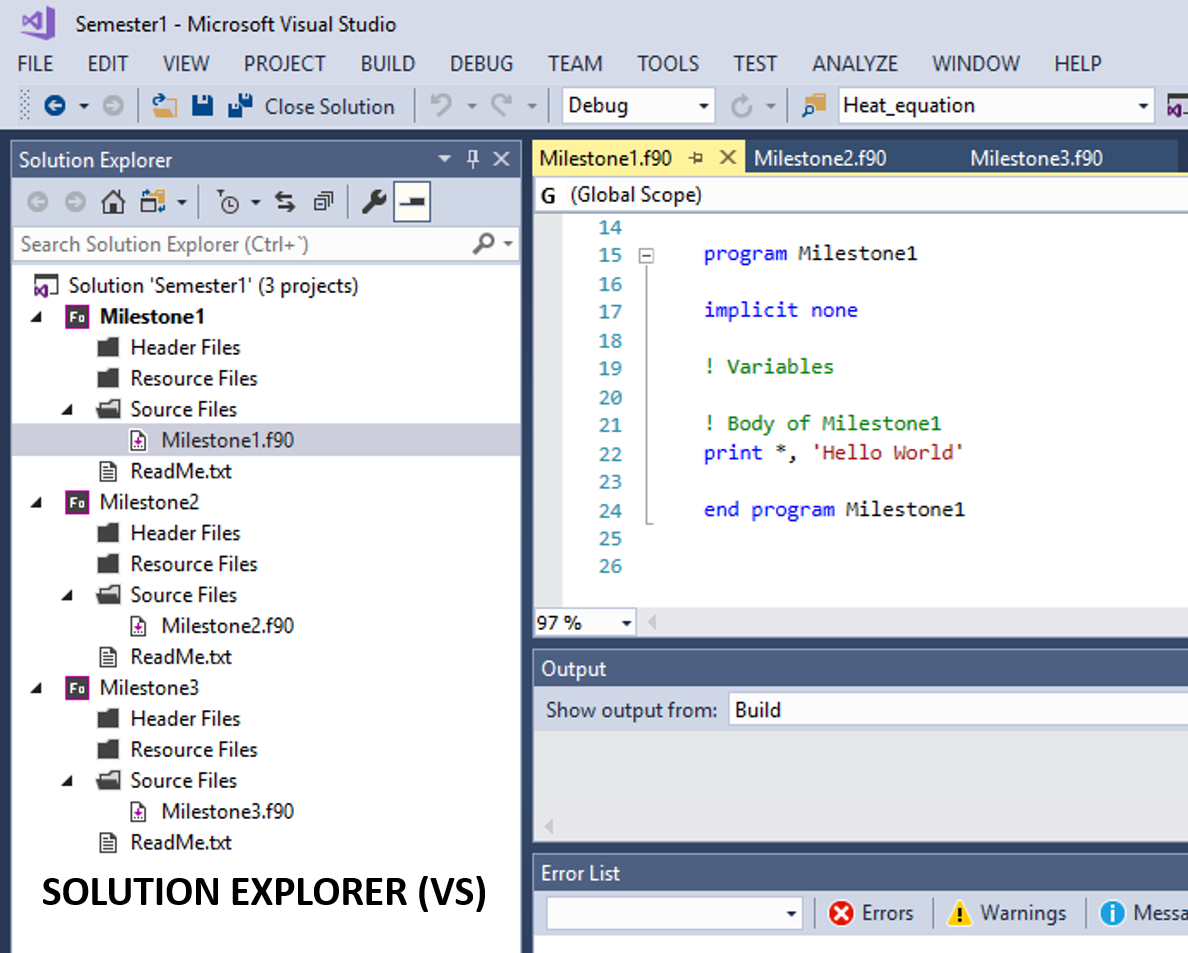
\includegraphics[width= \textwidth]{Figures/Intro4}
    \caption{Folders and files structure in the Solution Explorer of Visual Studio after creating three projects in the same solution.}
    \label{fig:Intro4}
\end{figure}





